\chapter[Neural networks for nonlinear SysId]{Neural Networks for Nonlinear System Identification}
\begin{quotation}
    \noindent
    \textsf{In \textbf{Part I} we have seen the Set-Membership approach for black-box identification of a dynamical system (linear, nonlinear, SISO or MIMO). In the literature there are other approaches which uses machine learning models such as \textit{Fully connected neural networks} and \textit{Recurrent Neural Networks}. In this chapter we will briefly introduce the topic of Neural Networks, and we will give some ideas on what are the models that can be used in the context of \textbf{nonlinear system identification}.}
\end{quotation}

\noindent
We have seen the SM-ID of nonlinear systems in very particular cases when the nonlinearities are block-structured in the overall system. This is a strong information on the system itself which, in turn, provides useful insights to face the problem in the framework of Set-Membership identification. However, there are many fields where such assumptions cannot be done since we are dealing with complex MIMO nonlinear systems! \textbf{Neural Networks} (NN) in this case are useful, since they have some nice properties (see \textit{Universal approximation theorem}).\\
Here our aim is to identify a \textit{MIMO Discrete Time dynamical system} of the kind:
\begin{equation} \label{eq:regressor_form}
    y_t=\mathcal{S}({
        y_{t-1}, ..., y_{t-n}, u_t,..., u_{t-n}
    })
\end{equation}
where $\mathcal{S}:
\underbrace{
    \mathbb{R}^p \times \dots \times \mathbb{R}^p
}_{n \text{ times}} \times \underbrace{
    \mathbb{R}^q \times \dots \times \mathbb{R}^q
}_{n \text{ times}} \to \mathbb{R}^p$ is a nonlinear function. In \Cref{eq:regressor_form} the function $\mathcal{S}$ is in the so-called \textit{regressor form} or \textit{input-output form}. For the identification, a set of experimentally collected input-output data are given:
\begin{equation*}
    \{u_t,\tilde{y}_t\}_{t=1}^N
\end{equation*} 
NNs are useful especially when the structure of $\mathcal{S}$ is assumed to be completely unknown, leading to a black-box model. In the following we are giving a description of neural-networks from a functional analysis point of view.
 
\section{Brief introduction to Neural Networks}
A \textbf{Neural network} is the composition of functions called \textbf{layers}. A layer $\ell_i$ is, in particular a function $\ell_i: \mathbb{R}^{\nu_i-1}\to\mathbb{R}^{\nu_i}$ defined by:
\begin{equation}\label{eq:FCNN}
    \alpha=\ell_i(x)\doteq\phi(W_i{x}+\beta_i)
\end{equation}
where $\nu_i$ is the output dimension of the $i$-th layer, also referred as the \textbf{number of neurons} of the i-th layer; $\alpha$ is the output of the layer; $x$ is the \textit{input of the layer}, while $W_i$ and $\beta_i$ are respectively the \textbf{weight matrix} and the \textbf{bias vector}, finally the $\phi$ is the \textbf{activation function} (a nonlinear function in general\footnote{
    Such a $\phi$ can be: a sigmoid, an hyperbolic tangent, a ReLU, or the identity (in the last layer).
}).\\
The \Cref{eq:FCNN} is the formulation of a single layer of the so-called \textit{fully-connected neural network}. A single \textit{hidden} layer is a function $\mathcal{N}:\mathbb{R}^{n_i}\to\mathbb{R}^{n_o}$. For example, for the second hidden layer the output (before passing through the activation function) is given by: 
\begin{equation}
    z=\mathcal{N}(x)=\ell_2 \ \circ \ \ell_1(x)=W_2 \text{ReLU}(W_1x+\beta_1)+\beta_2
\end{equation}
In general a NN composed of $L$ layers is the function
\begin{equation*}
    \begin{aligned}
        z&=\mathcal{N}(x)=\ell_L \ \circ \ \ell_{L-1} \ \circ \ \dots \circ \ \ell_2 \ \circ \ell_1(x)=\\
        &=W_L \phi (W_{L-1}\phi(...\phi(W_2\phi(W_1x+\beta_1)+\beta_2)+...)+ \beta_{L-1})+\beta_{L}
    \end{aligned}
\end{equation*}

\subsection{Why Neural Networks?}
There is a nice result on NN: the $L_2$-norm of the distance between the real $f$ and $\mathcal{N}$ can be made arbitrarily small, in this way the function $\mathcal{N}$ is a "good" approximator for $f$. This is what is stated in the so-called \textbf{Universal Approximation Theorem (Barron, 1993)}.

\begin{theorem}[\textit{Universal Approximation Theorem}]
    Consider a single-layer neural network $\mathcal{N}:\mathbb{R}^{n_i}\to\mathbb{R}^{n_o}$ with $n$ neurons and $\tanh$ or $\sigma$ activation function. Let $\Omega\subset\mathbb{R}^{n_i}$ be a compact set. The \textbf{approximation error} of any function $f:\Omega\to\mathbb{R}^{n_o}$ can be bounded as: 
    \begin{equation}
        \Vert f-\mathcal{N} \Vert_{L_2} \doteq
        \int_{\Omega} \bigg(
            \vert f(x) - \mathcal{N}(x) \vert \ dx 
        \bigg)^{1/2} \le
        \frac{C}{\sqrt{n}}
    \end{equation}
    where $C$ is a suitable constant dependent on the Fourier transform of $f$.
\end{theorem}
This vanilla-version of the Universal approximation theorem can be extended for both \textit{multi-layer networks} in presence of \textit{different activation function}. How you can see the higher the number of neurons the more accurate the approximation that $\mathcal{N}$ gives for $f$. The number of neurons $n$ is an \textit{hyperparameter} to tune, in the sense that trial and error procedure is needed in order to find it.\\
This was just to introduce in a "simple" way the topic of NN, but how they can be used for identifying a dynamical system? This is the topic of the next section.

\section{The NNARX model}
This was the first use of neural networks for system identification. The main idea is to \textit{replace $\mathcal{S}$} with a neural network $\mathcal{N}$. If the network is large enough then $\mathcal{N}\approx{\mathcal{S}}$. For the \textbf{true system}, where the data are not affected by noise, we have that:
\begin{align*}
    &\tilde{y}_{n+1}=\mathcal{S}(\tilde{y}_n,...,\tilde{y}_1,u_{n+1},...,u_1)\\
    &\tilde{y}_{n+2}=\mathcal{S}(\tilde{y}_n+1,...,\tilde{y}_2,u_{n+2},...,u_2)\\
    &  \quad  \vdots\\
    & \tilde{y}_{N}=\mathcal{S}(\tilde{y}_N-1,...,\tilde{y}_N-n,u_{N},...,u_N-n)
\end{align*}
that is a set of nonlinear equations where $\tilde{y}_t=y_t$. Replacing $\mathcal{S}$ with $\mathcal{N}_\theta$ we get a system of equations in the parameters 
\begin{equation}
    \theta\doteq[
        \text{vec}(W_1)^T, \beta_1^T,...,\text{vec}(W_L),\beta_L^T
    ]
\end{equation}
We are obtaining: 
\begin{align*}
    &\tilde{y}_{n+1}=\mathcal{N}_\theta(\tilde{y}_n,...,\tilde{y}_1,u_{n+1},...,u_1)+e_{n+1}\\
    &\tilde{y}_{n+2}=\mathcal{N}_\theta(\tilde{y}_n+1,...,\tilde{y}_2,u_{n+2},...,u_2)+e_{n+2}\\
    &  \quad  \vdots\\
    & \tilde{y}_{N}=\mathcal{N}_\theta(\tilde{y}_N-1,...,\tilde{y}_N-n,u_{N},...,u_N-n)+e_{N}
\end{align*}
where the noise and the mismatch between $\mathcal{S}$ and $\mathcal{N}$ can be modeled as the \textbf{equation-error} $e_t$, also called \textbf{one-step ahead prediction error}. The parameters can be found by solving the following unconstrained \textit{nonlinear least-squares problem}:

\begin{equation} \label{eq:NARX_opt}
    \arg\min_\theta \sum_{t=n+1}^N \Vert e_t \Vert_2^2 = 
    \arg \min_\theta \sum_{t=n+1}^N \Vert \tilde{y}_t - \mathcal{N}_\theta(\phi_t) \Vert_2^2
\end{equation}
where $\phi_t$ is the regressor. The problem is nonlinear, non-convex and high dimensional, that in general can be solved (to a local minimum) by using the gradient descent algorithm. Note that in \Cref{eq:NARX_opt} we are minimizing the one-step ahead prediction error, such a network is giving us \textit{very low performance} in \textbf{simulation}\footnote{
    This is the result of the model when the prediction of the output $\hat{y}$ are used in the regressor $\phi_t$. 
} since the dynamical part of the system is not explicitly taken into account.

\begin{figure}[h]
    \centering
    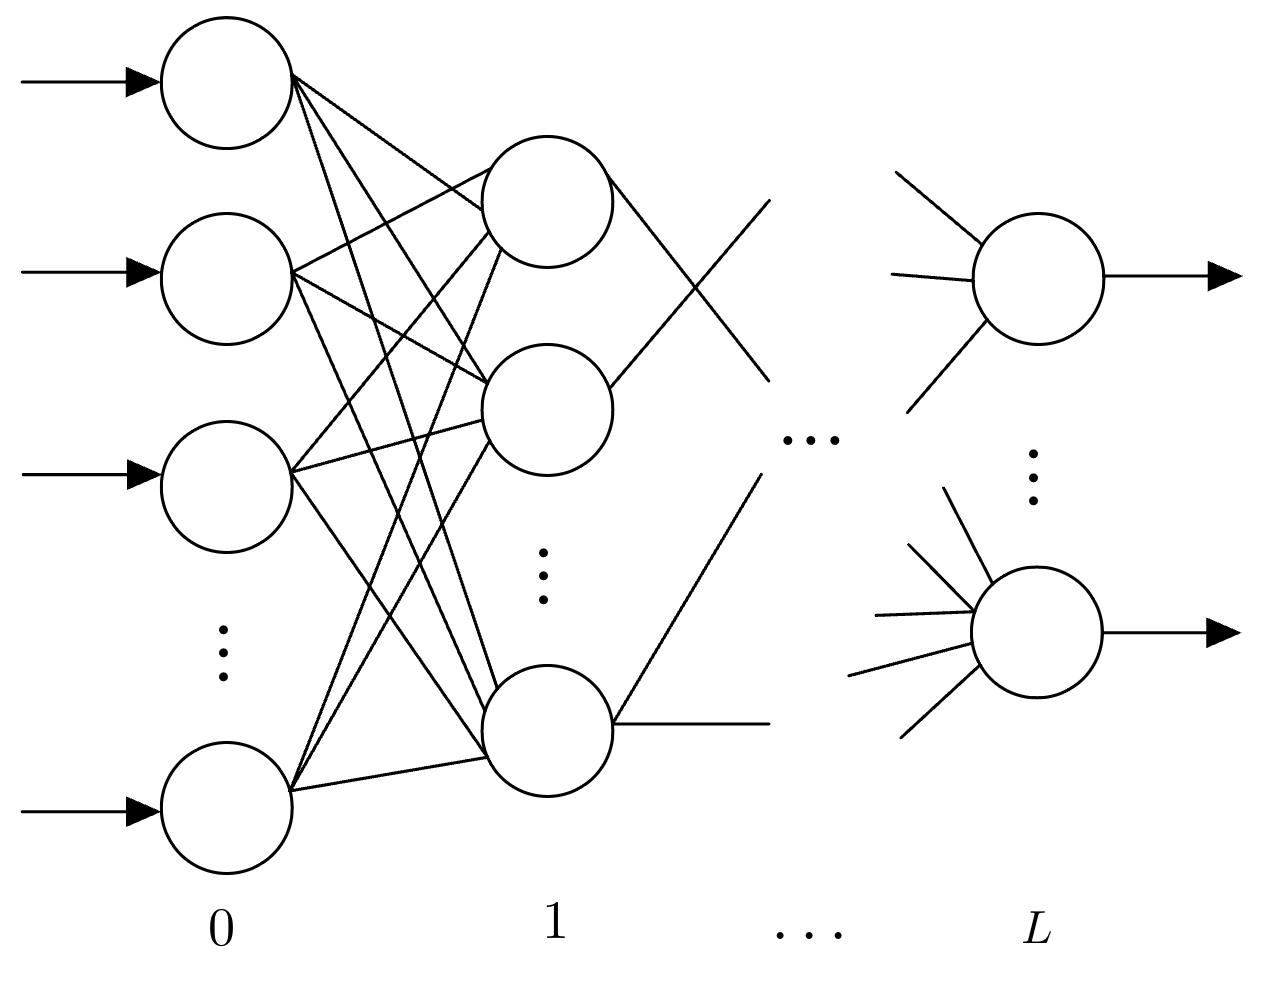
\includegraphics[scale=0.2]{img/NNARX.jpeg}
    \caption{Neural network used in the NNARX model}    
\end{figure}

\section{Recurrent Neural Networks (RNN)}
NNARX models use \textit{static NN} taking as input the whole regressor, bad performances are obtained in simulation, since there is not an explicit embedding of the dynamical part of the system in the neural model. A NN which contains the dynamics in its definition is called a \textbf{Recurrent Neural Network (RNN)}.

\subsection{Elman RNN}
This RNN model was introduced in the 90s. Here each layer $i$ of the RNN is a nonlinear state-space model with state $h^{(i)}$ of the kind
\begin{equation*}
    h_t^{(i)}=\phi(W_i x_t^{(i)} + V_i h_{t-1}^{(i)} + \beta_i)
\end{equation*}
where the term $V_i h_{t-1}^{(i)}$ makes a linear combination of the previous states. In the case the output and the state are the same. The first layer takes as input $x$ the input of the system $u$ while the hidden state $h$ is randomly initialized. The last layer that defines the output use the identity activation function.

\begin{figure}[h]
    \centering
    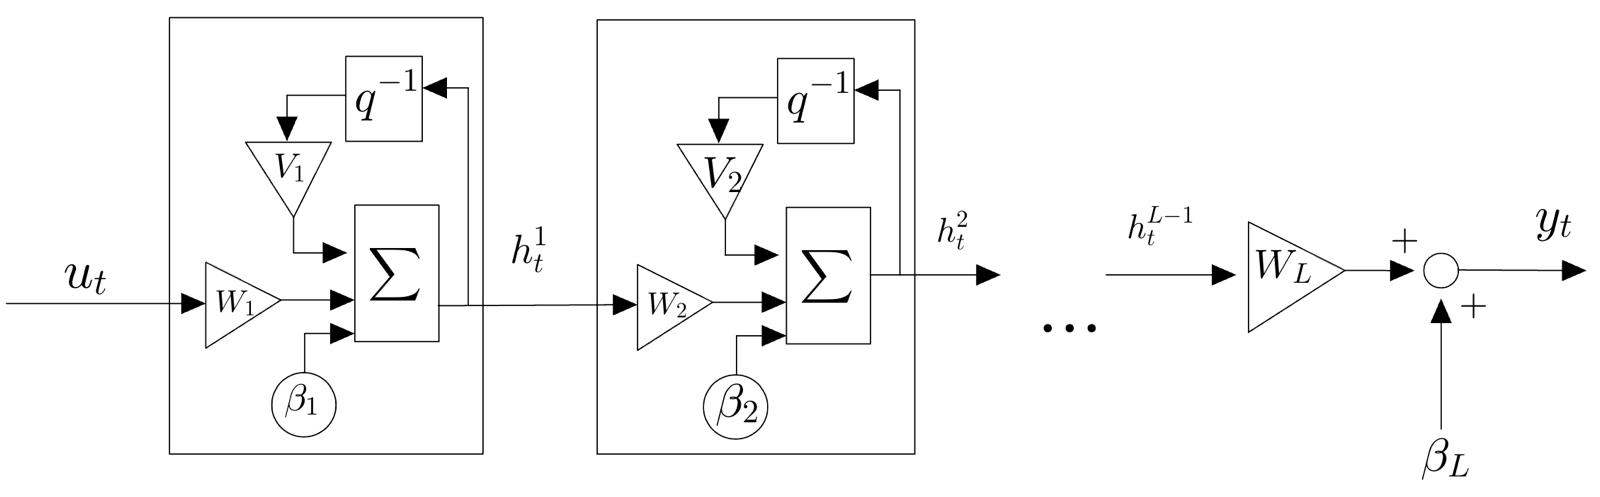
\includegraphics[scale=0.28]{img/RNN.jpeg}
    \caption{Elman RNN structure} 
\end{figure}

\subsection{Neural State-space models}
We know that, in discrete time, in general a nonlinear dynamical system can be represented in the \textbf{state-space form} as:
\begin{align*}
    x_{t+1}=f(x_t,u_t)\\
    y_t=h(x_t,u_t)
\end{align*}
a \textbf{neural state-space model} replace the nonlinear functions $f$ and $h$ with static NN $\mathcal{N}_f$ and $\mathcal{N}_h$, then: 
\begin{align*}
    x_{t+1}=\mathcal{N}_f([x_t^T,u_t^T]^T)\\
    y_t=\mathcal{N}_h([x_t^T,u_t^T]^T)
\end{align*}
the static NNs can have an arbitrary number of layers and neurons-per-layer. The difference here (that makes the overall architecture a recurrent one) is that the there is a feedback: the $x_t$ used are the one produced by $\mathcal{N}_f$. This is quite there is no $x$ in the collected data.

\subsection{Nonlinear Output Error models (NNOE)}
Is the dynamic counterpart of the NNARX model, with the only difference that here we use the \textit{predicted output} as input of the network instead of the collected data. It is defined by the recursive equation:
\begin{equation*}
    y_t=\mathcal{N}([y_{t-1}^T,...,y_{t-n}^T,u_t^T,...,u_{t-n}^T]^T)
\end{equation*}

\subsection{Training RNN and related issues}
Differently than the NNARX case, here the \textbf{simulation error} is minimized, that is the difference between the measured output and the one produced by the system. We have to solve the following optimization problem in order to retrieve the parameters $\theta$:
\begin{equation}
    \arg\min_{\theta} \underbrace{\sum_{t=1}^N{
        \Vert
            \tilde{y}_t - \hat{y}(u_t,x_0)
        \Vert_2^2}}_{\mathcal{L}(\theta)}
\end{equation}
where $\hat{y}(u_t,x_0)$ is the output of the RNN given the measured input $u_t$ and initial  conditions $x_0$ usually assumed to be randomly selected or zero. The functional $\mathcal{L}(\theta)$ is a strongly nonlinear function of the parameters. \\
Also in this case the gradient descent algorithm is used in order to solve the problem. Due to the dynamic nature of the problem the gradients $\nabla_\theta(\hat{y}_t)$ are related each other, this implicitly defines a dynamical system which is unstable as $t\to\infty$ and the gradients go to infinity, or it is asymptotically stable and the gradients are zero with the increasing time. These two conditions are called, respectively, \textbf{exploding} and \textbf{vanishing gradient issue}.\\
In order to tackle the issues related to the gradients computation, different models introducing a \textit{direct propagation path} for the gradients were introduced. We are talking about GRU (Gated Recurrent Units) and LSTM (Long-Short term memory) whose details are not discussed here.\\
Even if, there are such architectures the problems are attenuated but not fully solved, moreover a LSTM or a GRU requires \textbf{much more parameters} than standard RNN. To conclude this discussion, it is remarkable that the \textbf{Transformer} archicture are the best alternative to RNNs, but they are not suitable for system identification since the \textit{attention mechanisms} totally avoid the presence of an explicit feedback in the model.


\section{Modern trends}
What is the best way to avoid the issues related to the gradients? Avoiding to compute them! This is possible if we formulate the identification problem as a \textbf{constrained optimization problem} such as:
\begin{equation}
    \begin{aligned}
        &\arg \min_{\theta,y} \sum_{t=1}^N \Vert \tilde{y}_t - y_t \Vert_2^2\\
        &\text{s.t.} \ \tilde{y}_{n+1}=\mathcal{N}_\theta(\tilde{y}_n,...,\tilde{y}_1,u_{n+1},...,u_1), \ t=n+1,...,N
    \end{aligned}
\end{equation}

The resulting problem is more challenging from the computational point of view since it is constrained and has more variables. These results are presenteed in \citeauthor{cerone2024new}, \cite{cerone2024new} but are, of course, outside the scopes of this chapter.

\begin{figure}
    \centering
    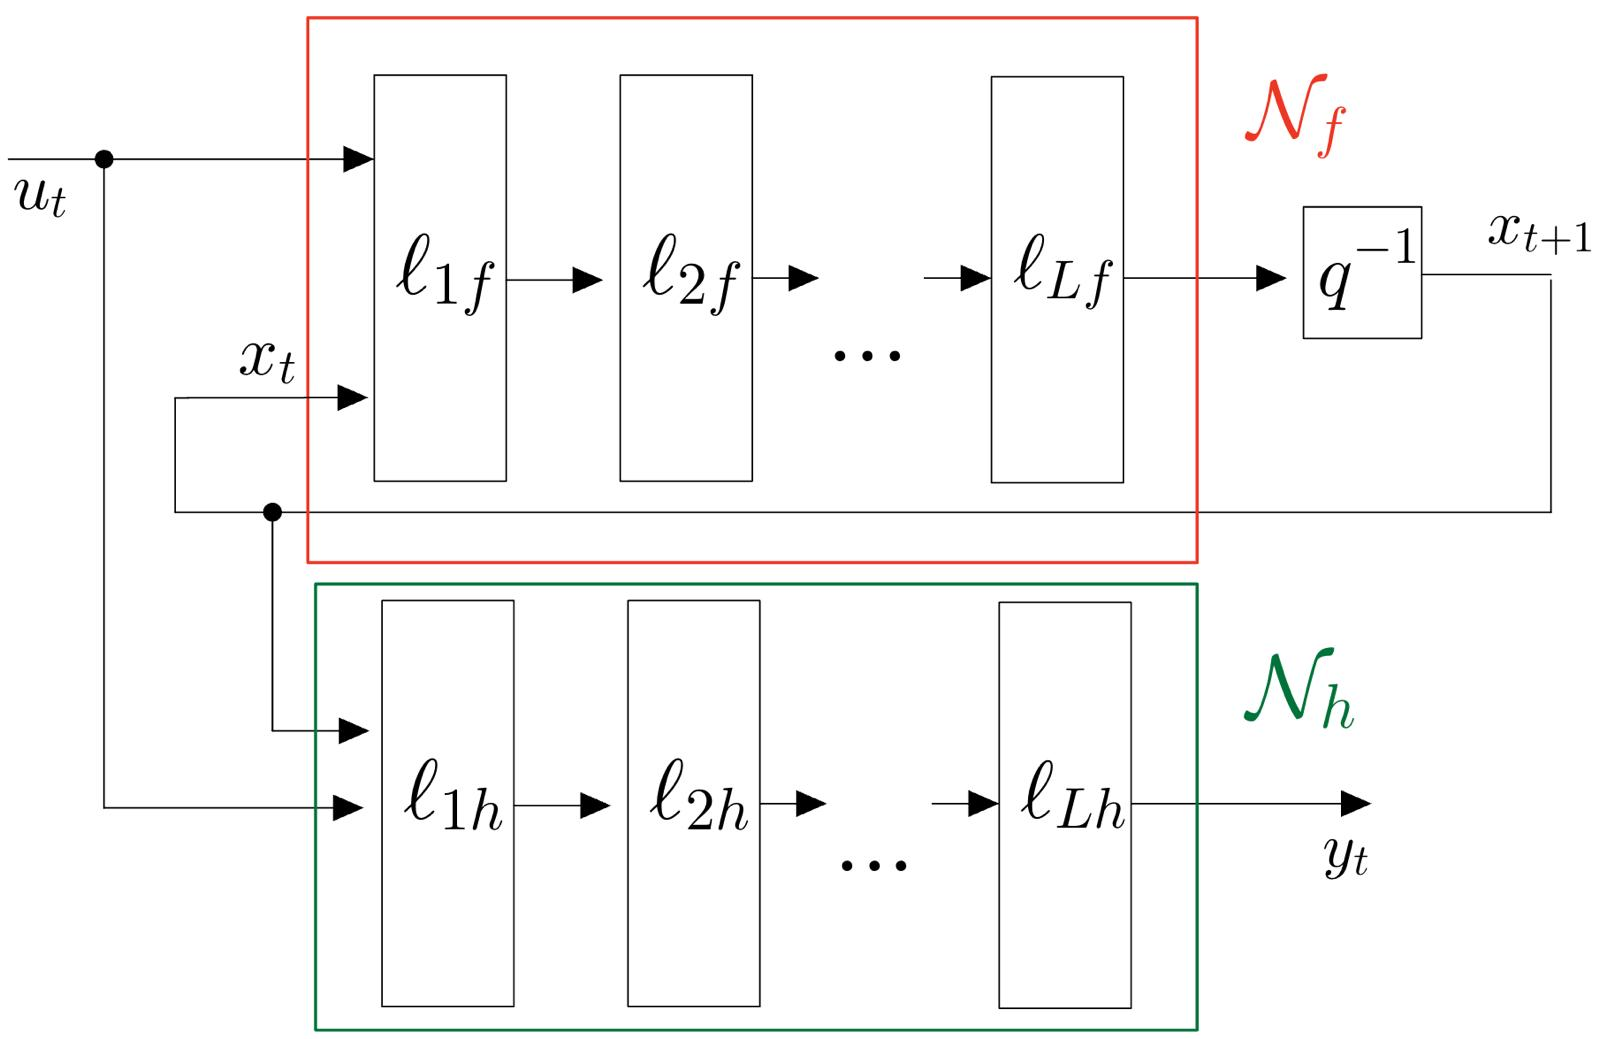
\includegraphics[scale=0.25]{img/NeuralSS.jpeg}
    \caption{Neural state-space model} 
\end{figure}

\begin{figure}
    \centering
    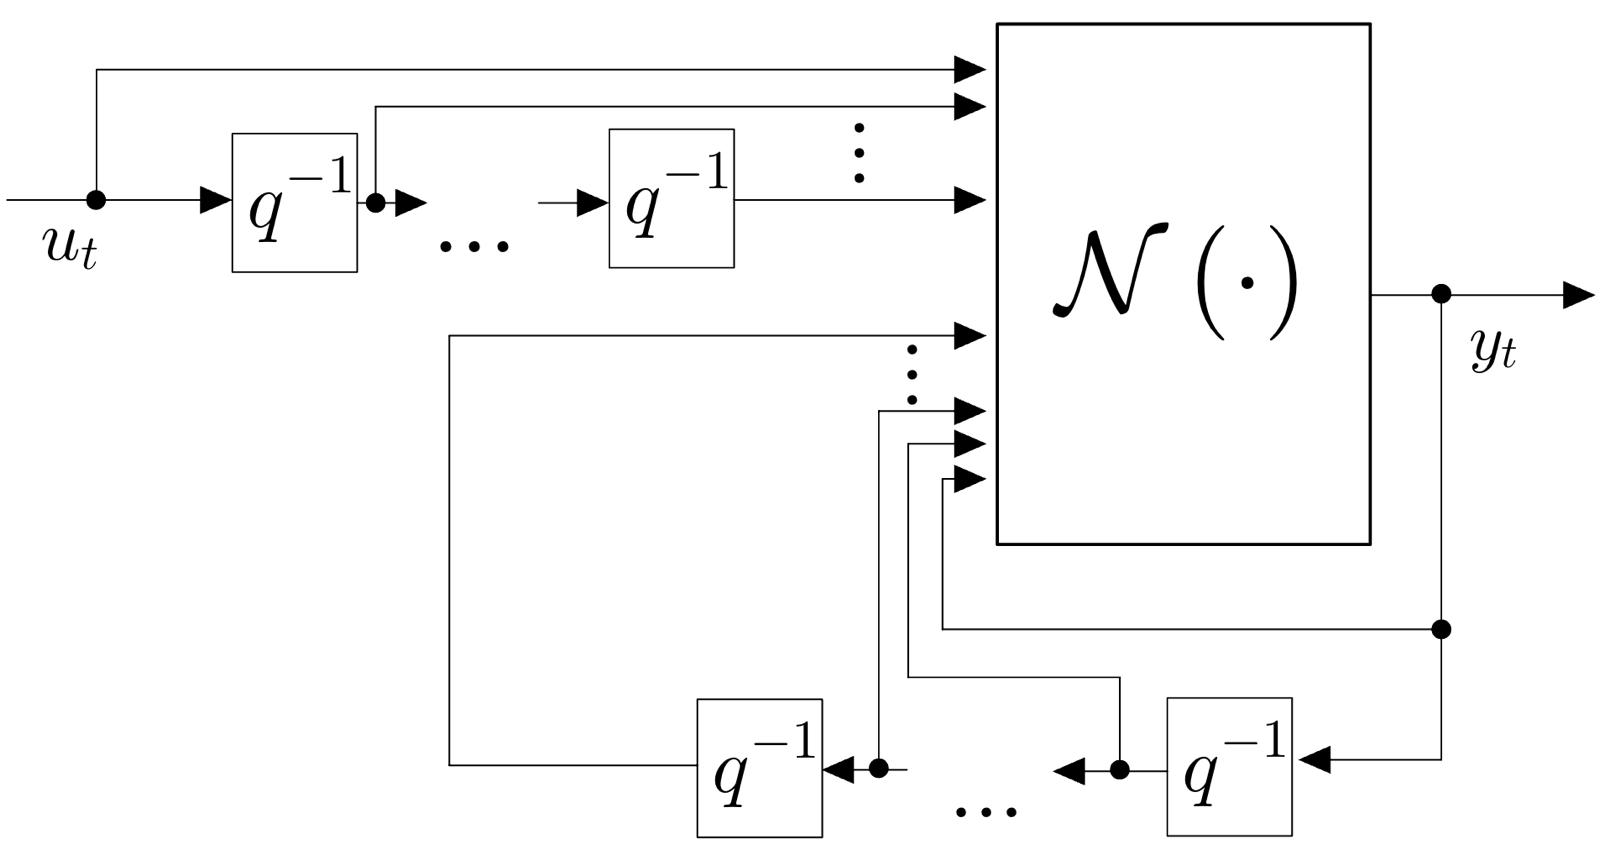
\includegraphics[scale=0.25]{img/NNOE.jpeg}
    \caption{NNOE structure} 
\end{figure}